\documentclass{article}
\usepackage{tikz, tkz-euclide}
\usepackage{circuitikz}
\usepackage{siunitx}
\usepackage[a5paper, margin=10mm, onecolumn]{geometry}
\usepackage{amsmath, amssymb, amsfonts}
\usepackage{graphicx}
\usepackage{xcolor}
\usepackage{mathrsfs}
\usepackage{pgfplots}
\usepackage{enumitem}
\usepackage{multicol}
\usepackage{mathtools}

% Define the custom commands
\newcommand{\brak}[1]{\left( #1 \right)}
\newcommand{\sbrak}[1]{\left[ #1 \right]}
\newcommand{\abs}[1]{\left| #1 \right|}
\newcommand{\lt}{<}
\newcommand{\gt}{>}
\begin{document}
\bibliographystyle{IEEEtran}
\title{ASSIGNMENT 15 GATE 2}of
\author{EE24BTECH11034 - K Teja Vardhan}
{\let\newpage\relax\maketitle}




    \begin{enumerate}
    \item Consider function $f(x) = (x^2 - 4)^2$ where $x$ is a real number. Then the function has 
        \begin{enumerate}
            \item only one minimum
            \item only two minima
            \item three minima
            \item three maxima
        \end{enumerate}

    \item Equation $e^x - 1 = 0$ is required to be solved using Newton's method with an initial guess $x_0 = -1$. Then, after one step of Newton's method, estimate $x_1$ of the solution will be given by  

        \begin{enumerate}
            \item 0.71828
            \item 0.36784
            \item 0.20587
            \item 0.00000
        \end{enumerate}

    \item $A$ is an $m \times n$ full rank matrix with $m > n$ and $I$ is an identity matrix. Let matrix $A^+ = (A^T A)^{-1} A^T$. Then, which one of the following statements is FALSE?
        \begin{enumerate}
            \item $AA^+A = A$
            \item $(AA^+)^2 = AA^+$
            \item $A^+A = I$
            \item $AA^+A = A^+$
        \end{enumerate}

    \item A differential equation $\frac{dx}{dt} = e^{-2t}u(t)$ has to be solved using the trapezoidal rule of integration with a step size $h = 0.01$ s. Function $u(t)$ indicates a unit step function. If $x(0-) = 0$, then the value of $x$ at $t = 0.01$ s will be given by:
        \begin{enumerate}
            \item 0.00099
            \item 0.00495
            \item 0.0099
            \item 0.0198
        \end{enumerate}

    \item Let $P$ be a $2 \times 2$ real orthogonal matrix and $\vec{x}$ is a real vector $[x_1, x_2]^T$ with length $|\vec{x}| = (x_1^2 + x_2^2)^{1/2}$. Then, which one of the following statements is correct?  

        \begin{enumerate}
            \item $|P\vec{x}| \leq |\vec{x}|$ where at least one vector satisfies $|P\vec{x}| < |\vec{x}|$
            \item $|P\vec{x}| = |\vec{x}|$ for all vectors $\vec{x}$
            \item $|P\vec{x}| \geq |\vec{x}|$ where at least one vector satisfies $|P\vec{x}| > |\vec{x}|$
            \item No relationship can be established between $|\vec{x}|$ and $|P\vec{x}|$
        \end{enumerate}

    \item Let $x(t) = rect(t - \frac{1}{2})$ where $rect(x) = 1$ for $-\frac{1}{2} \leq x \leq \frac{1}{2}$ and zero otherwise. Then if $\text{sinc}(x) = \frac{\sin(\pi x)}{\pi x}$, the Fourier Transform of $x(t) + x(-t)$ will be given by
        \begin{enumerate}
            \item $\text{sinc}(\frac{\omega}{2\pi})$
            \item $2\text{ sinc}(\frac{\omega}{2\pi})$
            \item $2\text{ sinc}(\frac{\omega}{2\pi}) \cos(\frac{\omega}{2})$
            \item $\text{sinc}(\frac{\omega}{2\pi}) \sin(\frac{\omega}{2})$
        \end{enumerate}

    \item Two perfectly matched silicon transistors are connected as shown in the figure. Assuming the $\beta$ of the transistors to be very high and the forward voltage drop in diodes to be  0.7V, the value of current $I$ is

        \begin{figure}[!ht]
        \centering
        \resizebox{0.7\textwidth}{!}{%
        \begin{circuitikz}
        \tikzstyle{every node}=[font=\small]
        \draw (10,11.75) to[Tnpn, transistors/scale=1.19] (10,9.25);
        \draw (13.5,9.25) to[Tpnp, transistors/scale=1.19] (13.5,11.75);
        \draw (10,9.25) to[short, -o] (14.5,9.25) ;
        \draw (13.5,11.75) to[short, -o] (13.5,12.25) ;
        \draw (11,10.5) to[short] (12.75,10.5);
        \draw (10,11.75) to[short] (11.75,11.75);
        \draw (11.75,11.75) to[short] (11.75,10.5);
        \draw (9.25,11.75) to[D] (10,11.75);
        \draw (8.25,11.75) to[R] (9.25,11.75);
        \draw (8.25,11.75) to (8,11.75) node[ground]{};
        \node [font=\small] at (8.75,12.25) {1 K$\Omega$};
        \node [font=\small] at (10,10.5) {Q1};
        \node [font=\small] at (13.5,10.5) {Q2};
        \draw [->, >=Stealth] (14,12.25) -- (14,11);
        \node [font=\small] at (14.25,11.75) {I};
        \node [font=\small] at (13.5,12.75) {+ 5V};
        \node [font=\small] at (15,9.25) {- 5V};
        \end{circuitikz}
        }%
        
        \label{fig:my_label}
        \end{figure}
        
        \begin{enumerate}
            \item 0 mA
            \item 3.6 mA
            \item 4.3 mA
            \item 5.7 mA
        \end{enumerate}

        
     \item A 230 V, 50 Hz, 4-pole, single-phase induction motor is rotating in the clockwise   (forward) direction at a speed of 1425 rpm. If the rotor resistance at standstill is 7.8  
      $\Omega$, then the effective rotor resistance in the backward branch of the equivalent circuit  will be
        \begin{enumerate}
            \item 2 $\Omega$
            \item 4 $\Omega$
            \item 7.8 $\Omega$
            \item 156 $\Omega$
        \end{enumerate}

    \item In the voltage doubler circuit shown in the figure, the switch 'S' is closed at \(t=0.\) Assuming diodes $D_1$ and $D_2$ to be ideal, load resistance to be infinite and initial capacitor voltages to be zero, the steady state voltage across capacitors  
    $C_1$ and $C_2$ will be  

    \begin{figure}[!ht]
    \centering
    \resizebox{1\textwidth}{!}{%
    \begin{circuitikz}
    \tikzstyle{every node}=[font=\small]
    \draw (6,14) to[sinusoidal voltage source, sources/symbol/rotate=auto] (6,11.75);
    \draw (6,14) to[closing switch] (7.5,14);
    \draw (7.5,14) to[curved capacitor] (8.25,14);
    \draw (8.25,14) to[D] (8.25,11.75);
    \draw (6,11.75) to[short] (8.25,11.75);
    \draw (10,14) to[D] (8.25,14);
    \draw (10,14) to[curved capacitor] (10,11.75);
    \draw (8.25,11.75) to[short] (10,11.75);
    \draw (10,14) to[short] (11.5,14);
    \draw (10,11.75) to[short] (11.5,11.75);
    \draw (11.5,14) to[R] (11.5,11.75);
    \draw [->, >=Stealth] (7.75,14.5) -- (6.25,14.5);
    \node [font=\small] at (5,12.75) {$5 sin \omega t$};
    \node [font=\small] at (6.75,13.75) {t = 0};
    \node [font=\small] at (6.25,14.25) {S};
    \node [font=\small] at (7.5,13.5) {C1};
    \node [font=\small] at (7.75,13) {D1};
    \node [font=\small] at (9,14.5) {D2};
    \node [font=\small] at (9.25,13) {C2};
    \node [font=\small] at (10.25,12.5) {Vc2};
    \node [font=\small] at (12.5,12.75) {R(load)};
    \end{circuitikz}
    }%
    
    \label{fig:my_label}
    \end{figure}
    
      \begin{enumerate}
            \item 2 $\Omega$
            \item 4 $\Omega$
            \item 7.8 $\Omega$
            \item 156 $\Omega$
        \end{enumerate}

    \item A 400 V, 50 Hz, 30 hp, three-phase induction motor is drawing 50 A current at 0.8 power factor lagging. The stator and rotor copper losses are 1.5 kW and 900 W respectively. The friction and windage losses are 1050 W and the core losses are 1200  
     W. The air-gap power of the motor will  
     be
        \begin{enumerate}
            \item 23.06 kW
            \item 24.11 kW
            \item 25.01 kW
            \item 26.21 kW
        \end{enumerate}

    \begin{figure}[!ht]
\centering
\resizebox{0.5\textwidth}{!}{%
\begin{circuitikz}
\tikzstyle{every node}=[font=\small]

\draw (12.25,10.5) to[short] (12.5,10.5);
\draw (12.25,10) to[short] (12.5,10);
\draw (12.5,10.5) node[ieeestd or port, anchor=in 1, scale=0.89](port){} (port.out) to[short] (14.25,10.25);
\draw (11.75,10.75) to[short, -o] (12.25,10.75) ;
\draw (11.75,9.75) to[short, -o] (12.25,9.75) ;
\draw (11.75,10.75) to[short] (11.75,11.25);
\draw (11.75,9.75) to[short] (11.75,9.25);
\draw (11.75,11.25) to[short, -o] (9.5,11.25) ;
\draw (12.25,10.5) to[short, -o] (9.5,10.5) ;
\draw (11.25,9.5) to[short, -o] (9.5,9.5) ;
\draw (11.75,9.25) to[short, -o] (9.5,9.25) ;
\draw (10.25,10.75) to[short, -o] (9.5,10.75) ;
\draw (11.25,10) to[short] (11.25,9.5);
\draw (11.25,10) to[short] (12.25,10);
\draw (10.25,10) to[short, -o] (9.5,10) ;
\draw (10.5,8.75) to[short, -o] (9.5,8.75) ;
\draw  (6.25,11.75) rectangle (9.25,8.25);
\draw [short] (5.25,11) -- (6.25,11);
\draw [short] (5.25,10.25) -- (6.25,10.25);
\draw [short] (5.25,9.5) -- (6.25,9.5);
\node [font=\small] at (5,9.5) {X};
\node [font=\small] at (5,10.25) {Y};
\node [font=\small] at (5,11) {Z};
\node [font=\small] at (6.5,11) {A0};
\node [font=\small] at (6.5,10.25) {A1};
\node [font=\small] at (6.5,9.5) {A2};
\node [font=\small] at (9,11.25) {1};
\node [font=\small] at (9,10.75) {2};
\node [font=\small] at (9,10.5) {3};
\node [font=\small] at (9,10) {4};
\node [font=\small] at (9,9.5) {5};
\node [font=\small] at (9,9.25) {6};
\node [font=\small] at (9,8.75) {7};
\node [font=\small] at (14.5,10.25) {F};
\end{circuitikz}
}%

\label{fig:my_label}
\end{figure}

    \item A 3 line to 8 line decoder, with active low outputs, is used to implement a 3-variable Boolean function as shown in the figure. The simplified form of Boolean function F(A,B,C) implemented in 'Product of Sum' form will be

        \begin{enumerate}
            \item $(X+Z).(\overline{X}+\overline{Y}+\overline{Z}).(Y+Z)$
            \item $(\overline{X}+\overline{Z}).(X+Y+Z).(\overline{Y}+\overline{Z})$
            \item $(\overline{X}+\overline{Y}+Z).(\overline{X}+Y+Z).(X+\overline{Y}+Z).(X+Y+\overline{Z})$
            \item $(\overline{X}+\overline{Y}+\overline{Z}).(\overline{X}+Y+\overline{Z}).(X+Y+Z).(X+\overline{Y}+\overline{Z})$
        \end{enumerate}
        


    \item The block diagrams of two types of half-wave rectifiers are shown in the figure. The transfer characteristics of the rectifiers are also shown within the block. It is desired to make full wave rectifier using above two half-wave rectifiers. The resultant circuit will be 

  
         \begin{figure}[!ht]
                \centering
                \resizebox{0.5\textwidth}{!}{%
                \begin{circuitikz}
                \tikzstyle{every node}=[font=\small]
                \draw (12.5,10) node[op amp,scale=1] (opamp2) {};
                \draw (opamp2.+) to[short] (11,9.5);
                \draw  (opamp2.-) to[short] (11,10.5);
                \draw (13.7,10) to[short](14,10);
                \draw (11,9.5) to (11,9) node[ground]{};
                \draw (10.25,10.5) to[short] (11,10.5);
                \draw (9,10.5) to[R] (10.25,10.5);
                \draw (9,9.5) to[R] (10.5,9.5);
                \draw (10.5,10.5) to[short] (10.5,9.5);
                \draw (11,10.5) to[short] (11,11.5);
                \draw (11,11.5) to[R] (13.25,11.5);
                \draw (13.25,11.5) to[short] (13.25,10);
                \draw  (8,10.75) rectangle (9,10.25);
                \draw  (8,9.75) rectangle (9,9.25);
                \draw [->, >=Stealth] (6.75,10.5) -- (7.75,10.5);
                \draw [->, >=Stealth] (7.25,9.5) -- (7.75,9.5);
                \draw [short] (7.25,9.5) -- (7.25,10.5);
                \node [font=\small] at (6.5,10.75) {Vin};
                \node [font=\small] at (7,12) {(A)};                
                \node [font=\small] at (8.5,10.5) {P};
                \node [font=\small] at (8.5,9.5) {Q};
                \node [font=\small] at (9.5,11) {R};
                \node [font=\small] at (9.75,10) {R};
                \node [font=\small] at (12,12) {R};
                \node [font=\small] at (14.5,10) {V0};
                \end{circuitikz}
                }%
                
                \label{fig:my_label}
                \end{figure}

        \begin{figure}[!ht]
                \centering
                \resizebox{0.5\textwidth}{!}{%
                \begin{circuitikz}
                \tikzstyle{every node}=[font=\small]
                \draw (12.5,10) node[op amp,scale=1] (opamp2) {};
                \draw (opamp2.+) to[short] (11,9.5);
                \draw  (opamp2.-) to[short] (11,10.5);
                \draw (13.7,10) to[short](14,10);
                \draw (10.25,10.5) to[short] (11,10.5);
                \draw (9,10.5) to[R] (10.25,10.5);
                \draw (9,9.5) to[R] (10.5,9.5);
                \draw (11,10.5) to[short] (11,11.5);
                \draw (11,11.5) to[R] (13.25,11.5);
                \draw (13.25,11.5) to[short] (13.25,10);
                \draw  (8,10.75) rectangle (9,10.25);
                \draw  (8,9.75) rectangle (9,9.25);
                \draw [->, >=Stealth] (6.75,10.5) -- (7.75,10.5);
                \draw [->, >=Stealth] (7.25,9.5) -- (7.75,9.5);
                \draw [short] (7.25,9.5) -- (7.25,10.5);
                \node [font=\small] at (6.5,10.75) {Vin};
                \node [font=\small] at (8.5,10.5) {P};
                \node [font=\small] at (8.5,9.5) {Q};
                \node [font=\small] at (9.5,11) {R};
                \node [font=\small] at (9.75,10) {R};
                \node [font=\small] at (12,12) {R};
                \node [font=\small] at (14.5,10) {V0};
                \node [font=\normalfont] at (6.5,12) {(B)};
                \draw [short] (10.5,9.5) -- (11,9.5);
                \draw (11,9.5) to[R] (11,8.25);
                \draw (11,8.25) to (11,8) node[ground]{};
                \end{circuitikz}
                }%
                
                \label{fig:my_label}
                \end{figure}     

        \begin{figure}[!ht]
            \centering
            \resizebox{0.5\textwidth}{!}{%
            \begin{circuitikz}
            \tikzstyle{every node}=[font=\small]
            \draw (12.5,10) node[op amp,scale=1] (opamp2) {};
            \draw (opamp2.+) to[short] (11,9.5);
            \draw  (opamp2.-) to[short] (11,10.5);
            \draw (13.7,10) to[short](14,10);
            \draw (10.25,10.5) to[short] (11,10.5);
            \draw (9,10.5) to[R] (10.25,10.5);
            \draw (9,9.5) to[R] (10.5,9.5);
            \draw (11,10.5) to[short] (11,11.5);
            \draw (11,11.5) to[R] (13.25,11.5);
            \draw (13.25,11.5) to[short] (13.25,10);
            \draw  (8,10.75) rectangle (9,10.25);
            \draw  (8,9.75) rectangle (9,9.25);
            \draw [->, >=Stealth] (6.75,10.5) -- (7.75,10.5);
            \draw [->, >=Stealth] (7.25,9.5) -- (7.75,9.5);
            \draw [short] (7.25,9.5) -- (7.25,10.5);
            \node [font=\small] at (6.5,10.75) {Vin};
            \node [font=\small] at (6.5,12) {(C)};
            \node [font=\small] at (8.5,9.5) {P};
            \node [font=\small] at (8.5,10.5) {Q};
            \node [font=\small] at (9.5,11) {R};
            \node [font=\small] at (9.75,10) {R};
            \node [font=\small] at (12,12) {R};
            \node [font=\small] at (14.5,10) {V0};
            \draw [short] (10.5,9.5) -- (11,9.5);
            \draw (11,9.5) to[R] (11,8.25);
            \draw (11,8.25) to (11,8) node[ground]{};
            \end{circuitikz}
            }%
            
            \label{fig:my_label}
            \end{figure}

        \begin{figure}[!ht]
            \centering
            \resizebox{0.5\textwidth}{!}{%
            \begin{circuitikz}
            \tikzstyle{every node}=[font=\small]
            \draw (10.25,10.5) to[short] (11,10.5);
            \draw (9,10.5) to[R] (10.25,10.5);
            \draw (9,9.5) to[R] (10.5,9.5);
            \draw  (8,10.75) rectangle (9,10.25);
            \draw  (8,9.75) rectangle (9,9.25);
            \draw [->, >=Stealth] (6.75,10.5) -- (7.75,10.5);
            \draw [->, >=Stealth] (7.25,9.5) -- (7.75,9.5);
            \draw [short] (7.25,9.5) -- (7.25,10.5);
            \node [font=\small] at (6.5,10.75) {Vin};
            \node [font=\small] at (6.5,12.75) {(D)};
            \node [font=\small] at (8.5,9.5) {P};
            \node [font=\small] at (8.5,10.5) {Q};
            \node [font=\small] at (9.5,11) {R};
            \node [font=\small] at (9.75,10) {R};
            \draw [short] (10.5,9.5) -- (11,9.5);
            \draw (9,12.75) to (9,12.25) node[ground]{};
            \draw (9,12.75) to[R,l={ \small R}] (10.5,12.75);
            \draw (10.5,12.75) to[R,l={ \small R}] (12,12.75);
            \draw (12.5,11) node[op amp,scale=1, yscale=-1 ] (opamp2) {};
            \draw (opamp2.+) to[short] (11,11.5);
            \draw  (opamp2.-) to[short] (11,10.5);
            \draw (13.7,11) to[short](14,11);
            \draw (11,10.5) to[short] (11,9.5);
            \draw (10.5,12.75) to[short] (10.5,11.5);
            \draw (10.5,11.5) to[short] (11,11.5);
            \draw (12,12.75) to[short] (12.75,12.75);
            \draw (12.75,12.75) to[short] (13.25,12.75);
            \draw (13.25,12.75) to[short] (13.25,11);
            \draw [->, >=Stealth] (14,11) -- (14.25,11);
            \node [font=\small] at (14.5,11) {V0};
            \end{circuitikz}
            }%
            
            \label{fig:my_label}
            \end{figure}

        \item The truth table of a monoshot shown in the figure is given in the table given below: Two monoshots, one positive edge triggered and other negative edge triggered, are connected as shown in the figure. The pulse widths of the two monoshots  
         outputs, $Q_1$ and $Q_2$, are $T_{ON1}$ and $T_{ON2}$, respectively. The frequency and the duty cycle of the signal at $Q_1$ will respectively be

        \begin{figure}[!ht]
        \centering
        \resizebox{0.9\textwidth}{!}{%
        \begin{circuitikz}
        \tikzstyle{every node}=[font=\small]
        \draw  (7.25,13) rectangle (9.75,10.5);
        \draw  (9.75,13) rectangle (12.25,10.5);
        \draw [short] (7.25,12.5) -- (12.25,12.5);
        \draw [short] (7.25,11.5) -- (12.25,11.5);
        \draw [short] (8.25,13) -- (8.25,10.5);
        \draw [short] (11,13) -- (11,10.5);
        \draw [->, >=Stealth] (9,11.75) -- (9,12.25);
        \draw [->, >=Stealth] (7.75,11.25) -- (7.75,10.75);
        \draw [short] (10.25,12.25) -- (10.25,11.75);
        \draw [short] (10.5,11.75) -- (10.5,12.25);
        \draw [short] (10.25,11.75) -- (10.5,11.75);
        \draw [short] (10,12.25) -- (10.25,12.25);
        \node [font=\small] at (10.5,12.75) {Q1};
        \draw [short] (10.5,12.25) -- (10.75,12.25);
        \draw [short] (11.25,11.75) -- (11.5,11.75);
        \draw [short] (11.5,11.75) -- (11.5,12.25);
        \draw [short] (11.5,12.25) -- (11.75,12.25);
        \draw [short] (11.75,12.25) -- (11.75,11.75);
        \draw [short] (11.75,11.75) -- (12,11.75);
        \draw [short] (10,11.25) -- (10.25,11.25);
        \draw [short] (10.25,11.25) -- (10.25,10.75);
        \draw [short] (10.25,10.75) -- (10.5,10.75);
        \draw [short] (10.5,10.75) -- (10.5,11.25);
        \draw [short] (10.5,11.25) -- (10.75,11.25);
        \draw [short] (11.25,10.75) -- (11.5,10.75);
        \draw [short] (11.5,10.75) -- (11.5,11.25);
        \draw [short] (11.5,11.25) -- (11.75,11.25);
        \draw [short] (11.75,11.25) -- (11.75,10.75);
        \draw [short] (11.75,10.75) -- (12,10.75);
        \node [font=\small] at (7.75,12) {0};
        \node [font=\small] at (9,11) {1};
        \node [font=\small] at (7.75,12.75) {X};
        \node [font=\small] at (9,12.75) {Y};
        \draw  (14.25,12.5) rectangle (16.75,10);
        \draw [short] (13.25,11.75) -- (14.25,11.75);
        \draw [short] (13.25,11) -- (14.25,11);
        \draw [short] (15.25,12.5) -- (15.25,13);
        \draw [short] (14.25,12.5) -- (14.25,13);
        \draw [short] (16.5,12.5) -- (16.5,13);
        \draw (14.25,13) to[R] (15.25,13);
        \draw (15.25,13) to[curved capacitor] (16.5,13);
        \draw (16.75,11.75) to[short] (17.75,11.75);
        \draw (16.75,10.75) to[short] (17.75,10.75);
        \node [font=\small] at (13,11.75) {X};
        \node [font=\small] at (13,11) {Y};
        \node [font=\small] at (14.75,13.5) {R};
        \node [font=\small] at (15.75,13.5) {C};
        \node [font=\small] at (18,11.75) {Q};
        \node [font=\small] at (18,10.75) {Q1};
        \end{circuitikz}
        }%
        
        \label{fig:my_label}
        \end{figure}

        
        
        \begin{figure}[!ht]
        \centering
        \resizebox{0.9\textwidth}{!}{%
        \begin{circuitikz}
        \tikzstyle{every node}=[font=\small]
        \draw  (14.25,12.5) rectangle (16.75,10);
        \draw [short] (13.25,11.75) -- (14.25,11.75);
        \draw [short] (13.25,11) -- (14.25,11);
        \draw [short] (15.25,12.5) -- (15.25,13);
        \draw [short] (14.25,12.5) -- (14.25,13);
        \draw [short] (16.5,12.5) -- (16.5,13);
        \draw (14.25,13) to[R] (15.25,13);
        \draw (15.25,13) to[curved capacitor] (16.5,13);
        \draw (16.75,11.75) to[short] (17.75,11.75);
        \draw (16.75,10.75) to[short] (17.75,10.75);
        \node [font=\small] at (13,11) {Y};
        \node [font=\small] at (14.75,13.5) {R};
        \node [font=\small] at (15.75,13.5) {C};
        \node [font=\small] at (17.25,12) {Q};
        \node [font=\small] at (17.25,10.5) {Q1};
        \node [font=\small] at (15.5,11.5) {$T(\text{on}) = 0.7 RC$};
        \draw  (22,12.5) rectangle (24.5,10);
        \draw [short] (21,11.75) -- (22,11.75);
        \draw [short] (21,10.75) -- (22,10.75);
        \draw [short] (23,12.5) -- (23,13);
        \draw [short] (22,12.5) -- (22,13);
        \draw [short] (24.25,12.5) -- (24.25,13);
        \draw (22,13) to[R] (23,13);
        \draw (23,13) to[curved capacitor] (24.25,13);
        \draw (24.5,11.75) to[short] (25.5,11.75);
        \draw (24.5,10.75) to[short] (25.5,10.75);
        \node [font=\small] at (21,12) {X};
        \node [font=\small] at (21,10.25) {Y};
        \node [font=\small] at (22.5,13.25) {R};
        \node [font=\small] at (23.75,13.5) {C};
        \node [font=\small] at (23.5,11.25) {$T(\text{on}) = 0.7 RC$};
        \draw (17.75,10.75) to[short] (21.5,10.75);
        \draw (21,11.75) to (20.75,11.75) node[ground]{};
        \draw (13.25,11.75) to[short] (12.5,11.75);
        \draw (26,11.75) to[short] (25.5,11.75);
        \draw (12.5,11.75) to[short] (12.5,9);
        \draw (12.5,9) to[short] (26,9);
        \draw (26,11.75) to[short] (26,9);
        \node [font=\small] at (25,11) {$Q'_2$};
        \node [font=\small] at (25,12) {$Q_2$};
        \end{circuitikz}
        }%
        \label{fig:my_label}
        \end{figure}

    \begin{enumerate}
            \item $f = \frac{1}{T_{ON_1} + T_{ON_2}}, \quad D = \frac{T_{ON_1}}{T_{ON_1} + T_{ON_2}}$
            \item $f = \frac{1}{T_{ON_1} + T_{ON_2}}, \quad D = \frac{T_{ON_2}}{T_{ON_1} + T_{ON_2}}$
            \item $f = \frac{1}{T_{ON_1}}, \quad D = \frac{T_{ON_1}}{T_{ON_1} + T_{ON_2}}$
            \item $f = \frac{1}{T_{ON_2}}, \quad D = \frac{T_{ON_1}}{T_{ON_1} + T_{ON_2}}$
        \end{enumerate}

    \item The contents (in Hexadecimal) of some of the memory locations in an 8085A based system are given below:

    \begin{tabular}{|c|c|}
        \hline
        Address & Contents \\
        \hline
        ... & ... \\
        26FE & 00 \\
        26FF & 01 \\
        2700 & 02 \\
        2701 & 03 \\
        2702 & 04 \\
        ... & ... \\
        \hline
    \end{tabular}

    The contents of stack pointer (SP), program counter (PC) and (H.L) are 2700H, 2100H and 0000H respectively. When the following sequence of instructions  
 are executed,

    assembly
    2100 H:  DAD SP ;
    2101 H:  PCHL
    

    the contents of (SP) and (PC) at the end of execution will be
        \begin{enumerate}
            \item (PC) = 2102H, (SP) = 2700H
            \item (PC) = 2700H, (SP) = 2700H
            \item (PC) = 2800H, (SP) = 26FEH
            \item (PC) = 2A02H, (SP) = 2702H
        \end{enumerate}

     \item A waveform generator circuit using OPAMPs is shown in the figure. It produces a triangular wave at point 'P' with a peak to peak voltage  
        of 5 V for $v_i = 0$ V. If the voltage v, is made +2.5V, the voltage waveform at point 'P' will become

    \begin{figure}[!ht]
        \centering
        \resizebox{0.6\textwidth}{!}{%
        \begin{circuitikz}
        \tikzstyle{every node}=[font=\small]
        \draw (14.75,10.5) node[op amp,scale=1] (opamp2) {};
        \draw (opamp2.+) to[short] (13.25,10);
        \draw  (opamp2.-) to[short] (13.25,11);
        \draw (15.95,10.5) to[short](16.25,10.5);
        \draw (23,10.5) node[op amp,scale=1] (opamp2) {};
        \draw (opamp2.+) to[short] (21.5,10);
        \draw  (opamp2.-) to[short] (21.5,11);
        \draw (24.2,10.5) to[short](24.5,10.5);
        \draw (16.25,10.5) to[short] (17,10.5);
        \draw (17,10.5) to[short] (17.5,10.5);
        \draw (17.5,10.5) to[short] (17.5,11);
        \draw (17.5,11) to[R] (21.5,11);
        \draw (21,11) to[short] (21,12);
        \draw (21,12) to[curved capacitor] (23.75,12);
        \draw (23.75,12) to[short] (23.75,10.5);
        \draw (17.5,9) to[empty Schottky diode] (17.5,10);
        \draw (17.5,10.5) to (17.5,10.25) node[sground]{};
        \draw (17.5,9) to (17.5,8.75) node[ground]{};
        \draw (16.25,10.5) to[short] (16.25,8.75);
        \draw (16.25,8.75) to[R] (14,8.75);
        \draw (13.25,10) to[short] (13.25,8.75);
        \draw (13.25,8.75) to[short] (14,8.75);
        \draw (13.25,8.75) to[R] (13.25,7.5);
        \draw (13.25,7.5) to[short] (24,7.5);
        \draw (24,10.5) to[short] (24,7.5);
        \draw (13.25,11) to (12.5,11) node[ground]{};
        \node [font=\small] at (15,9.25) {R1};
        \node [font=\small] at (13.75,8) {R1};
        \node [font=\small] at (19.5,11.5) {R};
        \draw (20,8.75) to[R] (23,8.75);
        \draw (23,8.75) to[short] (23,8.25);
        \draw (20,8.75) to[short] (20,8.25);
        \draw [->, >=Stealth] (21.5,10) -- (21.5,9);
        \node [font=\small] at (21.75,9.5) {V1};
        \node [font=\small] at (20,8) {+12 V};
        \node [font=\small] at (23,8) {-12 V};
        \node [font=\small] at (24.75,10.5) {P};
        \end{circuitikz}
        }%
        
        \label{fig:my_label}
        \end{figure}

    \begin{figure}[h!]
    \centering
      \hspace{-1cm}
      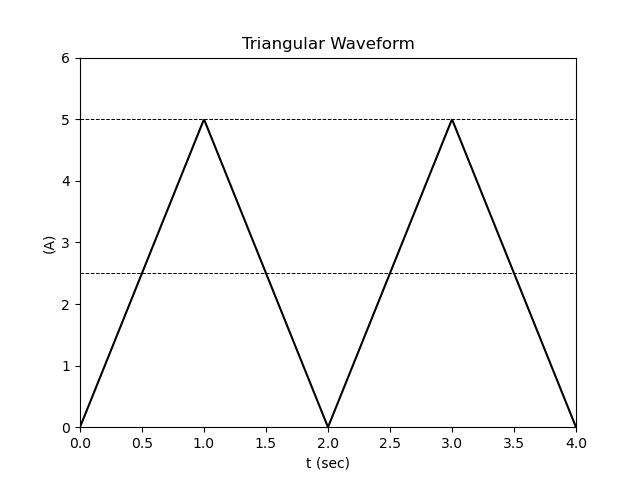
\includegraphics[width=0.375\textwidth]{Figure_1.png}
      
      \caption{Option A }
      \label{fig:your_label}
    \end{figure}

    \begin{figure}[h!]
    \centering
      \hspace{-1cm}
      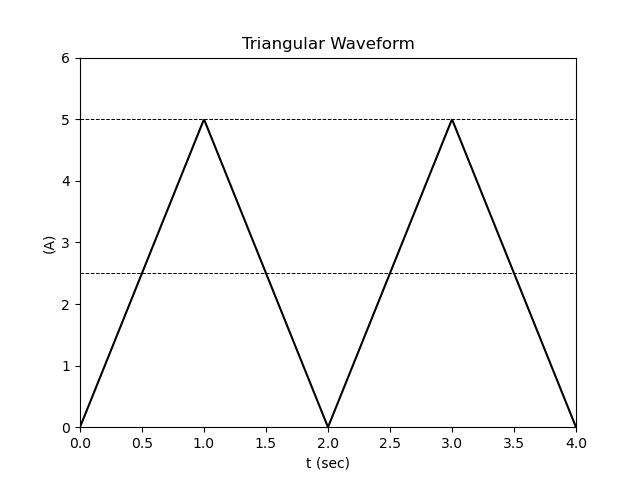
\includegraphics[width=0.375\textwidth]{Figure_1.png}
      
      \caption{Option B }
      \label{fig:your_label}
    \end{figure}

    \begin{figure}[h!]
    \centering
      \hspace{-1cm}
      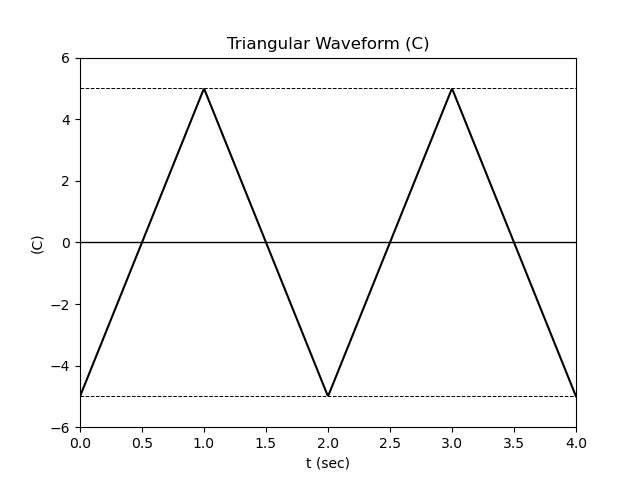
\includegraphics[width=0.375\textwidth]{Figure_3.png}
      
      \caption{Option C }
      \label{fig:your_label}
    \end{figure}

    \begin{figure}[h!]
    \centering
      \hspace{-1cm}
      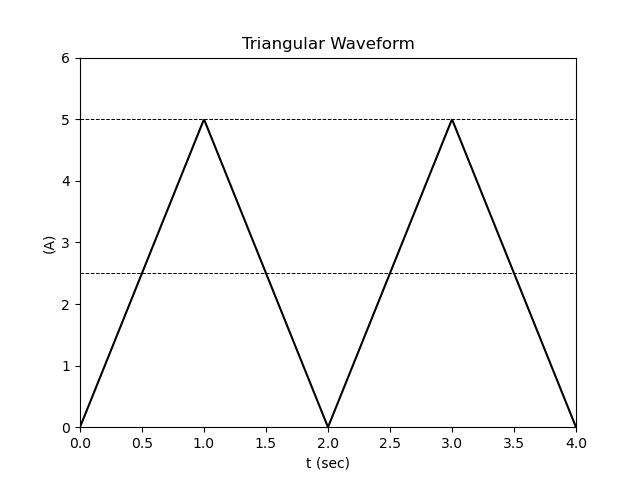
\includegraphics[width=0.375\textwidth]{Figure_1.png}
      \caption{Option D}
      \label{fig:your_label}
    \end{figure}

    \item Voltage phasors at the two terminals of a transmission line of length 70 km have a magnitude of 1.0 per unit but are 180 degrees out of phase. Assuming that the maximum load current in the line  
 is 1/5th of minimum 3-phase fault current, which one of the following transmission line protection schemes will NOT pick up for this condition?  

        \begin{enumerate}
            \item Distance protection using mho relays with zone-1 set to 80% of the line impedance
            \item Directional overcurrent protection set to pick up at 1.25 times the maximum load current
            \item Pilot relaying system with directional comparison scheme
            \item Pilot relaying system with segregated phase comparison scheme
        \end{enumerate}

    \item A lossless transmission line having Surge Impedance Loading (SIL) of 2280 MW is provided with a uniformly distributed series capacitive compensation of  
 30 %. Then, SIL of the compensated transmission line will be  

        \begin{enumerate}
            \item 1835 MW
            \item 2280 MW
            \item 2725 MW
            \item 3257 MW
        \end{enumerate}       


     \item The core of a two transformer is subjected to a magnetic flux variation as indicated in the figure. the induced EMF in the secondary winding as a function of time will be in the form.

   \begin{figure}[h!]
    \centering
      \hspace{-1cm}
      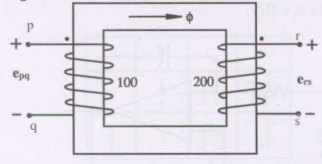
\includegraphics[width=0.5\textwidth]{Screenshot from 2024-10-26 12-11-33.png}
      
      \label{fig:your_label}
    \end{figure}

    \begin{figure}[h!]
    \centering
      \hspace{-1cm}
      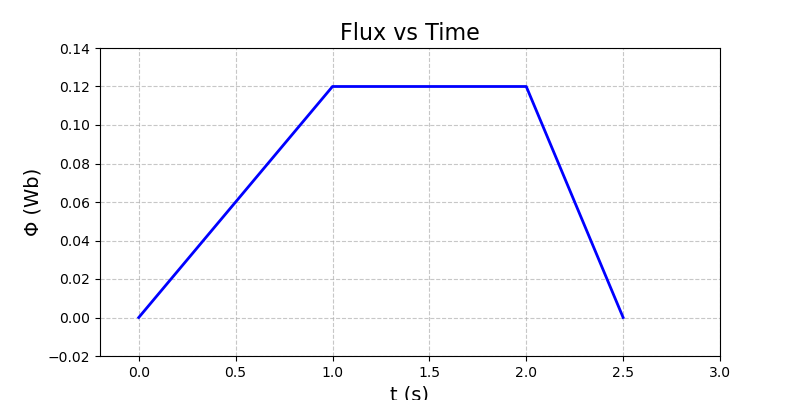
\includegraphics[width=0.5\textwidth]{Figure_4.png}
      \caption{OPTIONS ARE GIVEN BELOW}
      \label{fig:your_label}
    \end{figure}


    \begin{figure}[h!]
    \centering
      \hspace{-1cm}
      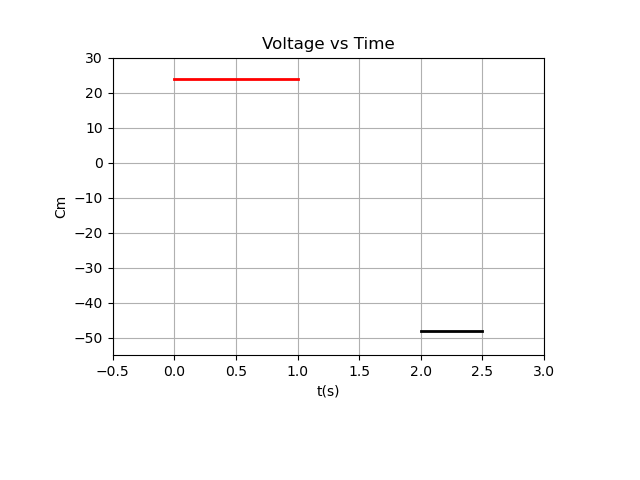
\includegraphics[width=0.7\textwidth]{Figure_6.png}
      \caption{A}
      \label{fig:your_label}
    \end{figure}

   \begin{figure}[h!]
    \centering
      \hspace{-1cm}
      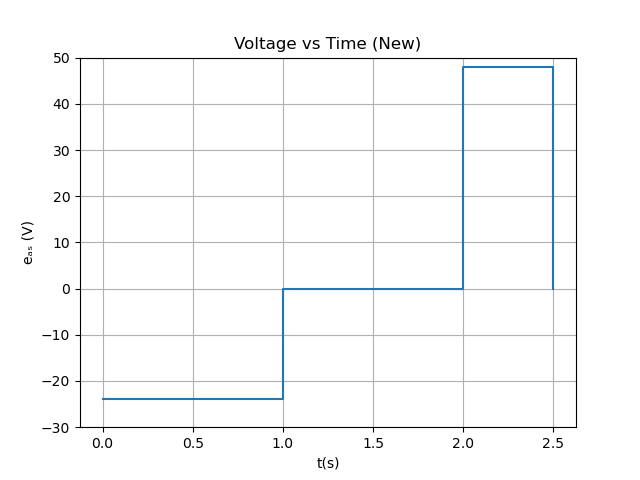
\includegraphics[width=0.5\textwidth]{Figure_7.png}
      \caption{B}
      \label{fig:your_label}
    \end{figure}

    \begin{figure}[h!]
    \centering
      \hspace{-1cm}
      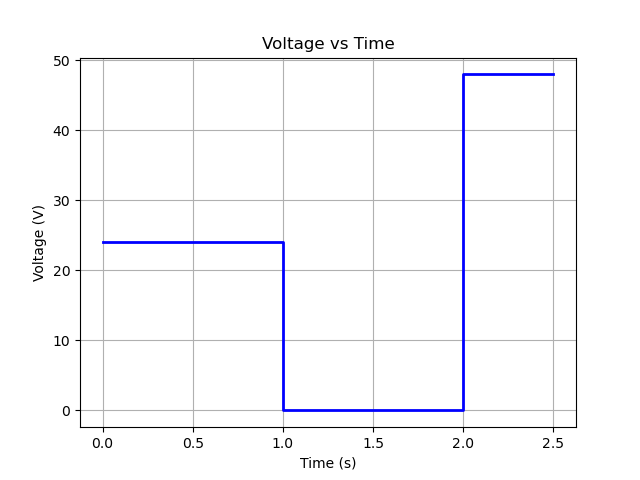
\includegraphics[width=0.5\textwidth]{Figure_8.png}
      \caption{C}
      \label{fig:your_label}
    \end{figure}

    \begin{figure}[h!]
    \centering
      \hspace{-1cm}
      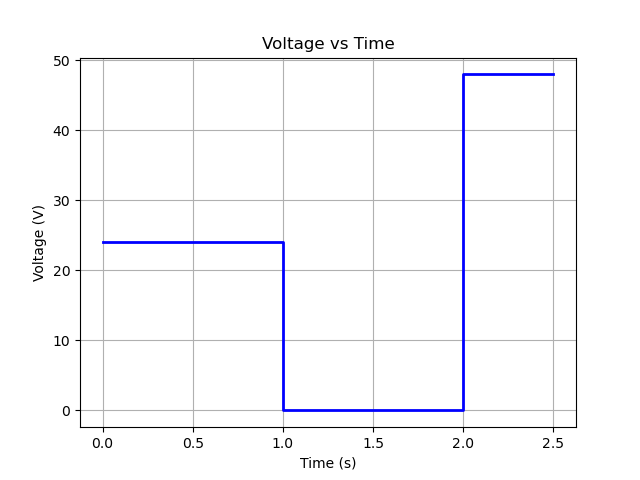
\includegraphics[width=0.5\textwidth]{Figure_5.png}
      \caption{D}
      \label{fig:your_label}
    \end{figure}

    
    


   
   
\end{enumerate}
\end{document}
